\documentclass{article}
% load packages
\usepackage{amsmath}
\usepackage{amssymb}
\usepackage{hyperref}
\usepackage{graphicx}
% setup bibliography
\usepackage[style=numeric,backend=biber]{biblatex}
\addbibresource{aggregation.bib}

\renewcommand{\vec}[1]{\boldsymbol{#1}}

% ----------------------------- %
\title{Aggregation by Movement}
\author{Ole Schügl}
% ----------------------------- %
\begin{document}
\maketitle

\section{Introduction}
Spatial pattern formation is a fascinating phenomenon that can be observed in a wide range of ecosystems, such as mussel beds and arid bushlands \autocite{liuPhaseSeparationDriven2016,rietkerkSelfOrganizationVegetationArid}. 
There is evidence that the stability of these ecosystems is improved by spatial patterns, for example in mussel beds through improved nutrient availability while reducing the impact of disturbances due to water flow \autocite{vandekoppelExperimentalEvidenceSpatial2008}.

When modeling ecological systems, explicitly incorporating space can have qualitative impacts on the behaviour of the system. 
This was shown in ref. \cite{durrettImportanceBeingDiscrete1994}, where four different approaches for modeling the same system, two spatial models, and two non-spatial models, under three parameter choices were analysed and it was shown that no two models agree for all three parameter choices.
These results highlight the importance of selecting the right level of detail for modeling and being explicit about the assumptions, as well as understanding the conditions under which these assumptions hold.
Ordinary differential equations, for instance,  make the implicit assumption that the system under consideration is well-mixed. 
For the systems mentioned in the first paragraph, this assumption does not hold and it is necessary to model space explicitly.  

To explain the formation of the observed patterns, usually one of two mechanisms is put forward.
The first mechanism is based on the activation-inhibition principle described by Alan Turing \autocite{turingChemicalBasisMorphogenesis1952}.

The second mechanism is based on the lesser known phase-separation priniciple developed by Cahn and Hilliard. 
In ecological settings, this corresponds to density-dependent movement leading to pattern formation, as opposed to birth and death processes. A number of organisms, among them certain species of mussels, slime moulds and ants, whose spatial distribution can be explained by density-dependent movement is presented in \autocite{liuPhaseSeparationDriven2016}.


In this report, the spatial aggregation of individuals based on density-dependent movement in continuous space will be explored.
More specifically, we will look at a very simple but counter-intuitive mechanism that leads to aggregation, in which particles move faster when the local density is higher. 


\section{The Model}
First, a model for the density-dependent movement of organisms will be presented. 
The model 
The organisms will be simulated on a square with sidelength $1$ and periodic boundary conditions, which effectively means that organisms exist on a torus.
This is important to ensure that they are contained to a small region and makes it easier to visualize.

Since the focus is on movement, the number of organisms, $N$, is constant.
Initially, the organisms are distributed randomly in the environment. 
The position of all organisms is then updated at discrete time-steps by drawing a displacement from a normal distribution.
Mathematically, the change of the position $\vec{r}_i = (x_i, y_i)$ of individual $i$ can be described by
\begin{align}
    & x_i(t + dt) = x_i(t) + \sqrt{2D(N_R(\vec{r}_i, t)) dt} u_{i,x} \\
    & y_i(t + dt) = y_i(t) + \sqrt{2D(N_R(\vec{r}_i, t)) dt} u_{i,y}
\end{align}
where $u_{i,x}$ and $u_{i,y}$ are independent, normally distributed random numbers $\sim \mathcal{N}(0,1)$ and $D(N_R(\vec{r}_i, t))$ is a density-dependent diffusion rate.
The argument $N_R(\vec{r}_i, t)$ is the number of other organisms within a radius $R$ around the particle. 
For the diffusion rate function, we will use
\begin{equation}
    D(N_R(\vec{r}_i, t)) = D_0\left( \frac{N_R(\vec{r}_i, t)}{N\pi R^2} \right)^p.
\end{equation}
For a fixed interaction radius $R=0.1$, there are three parameters that influence the diffusion rate: $p, N$ and $D_0$.
In Fig. \ref{diffusion_rates}, the standard deviation of the increments as a function of the number of neighbours $\sigma(N_r) = \sqrt{2D(N_R) dt}$ is shown for a couple of different parameter values.
It can be seen, that the diffusion rate increases with the number of organisms in the neighbourhood.
Depending on the parameter $p$, this increase can be linear ($p=2$) or grow polynomially ($\mathcal{O}(n^{p/2})$). 
The parameter $D_0$ shifts the curves up or down, and could be understood as a baseline diffusion rate.

In simulations, the effects of these parameters on the spatial distribution will be analysed, but before that, a simpler setting will be discussed for comparison.
\begin{figure}
    \label{diffusion_rates} 
    \centering
    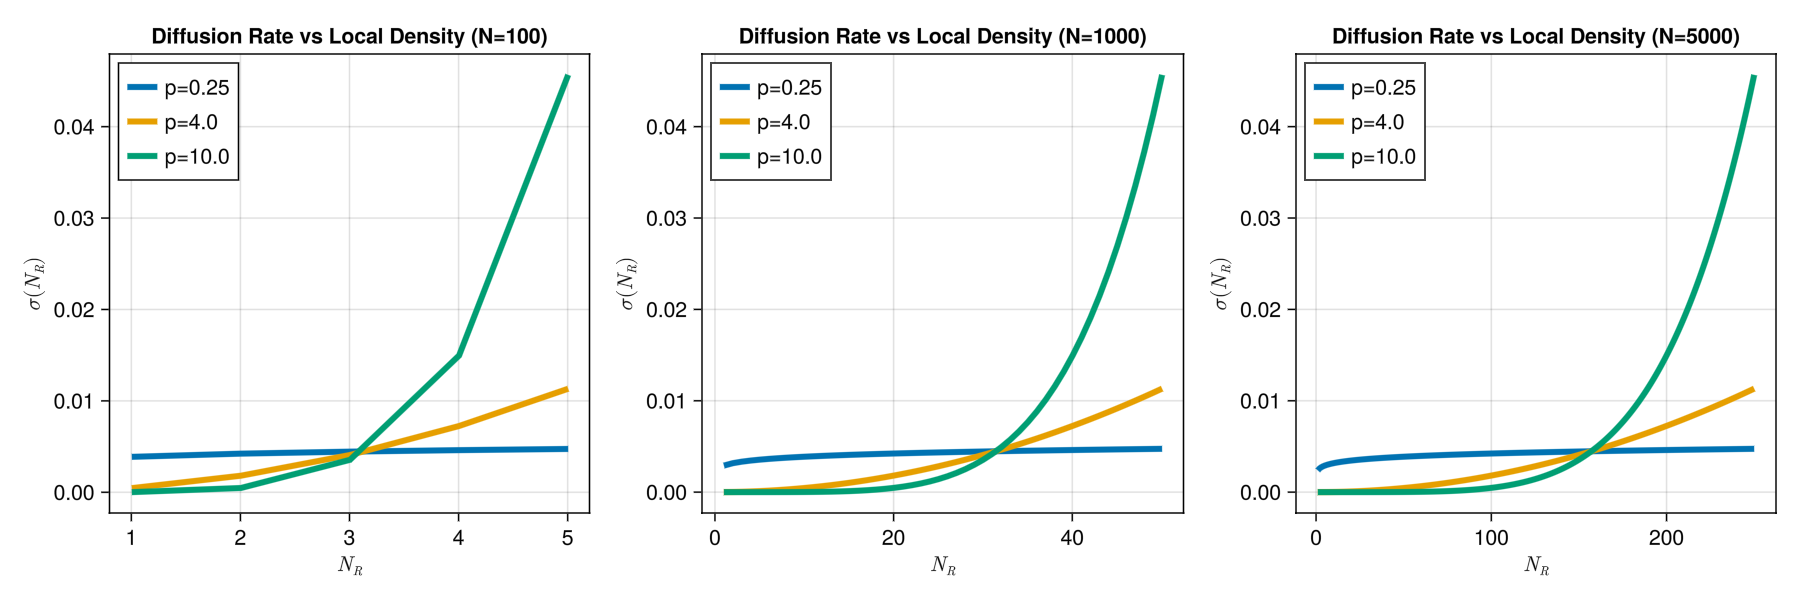
\includegraphics[width=1.0\linewidth]{img/diffusion_rates.png}
    \caption{Diffusion rate of an organism based on the number of other organisms within distance $R$ for $N=100$, $N=1000$, $N=5000$ and $p=0.25$, $p=4$, $p=10$ and $D_0 = 0.001$. Note that while the shape of the curves is the same, the number of organisms that can be within the radius to reach a certain diffusion rate increases with the total number of organisms.}
\end{figure}

\subsection{A Single Organism}
Before moving on to the simulations, the diffusion of a single organism in space will be analysed.

To do this, we consider a simple environment with only a single organism and a constant diffusion term. 
This can be recovered from the density-dependent diffusion rate by setting $p=0$.
For simplicity, it will be assumed that the environment is infinite, as opposed to the torus used in the simulations.\\
The walker position will change similiarly to before, but with a constant diffusion term
\begin{align}
    & x(t + dt) = x(t) + \sqrt{2D dt} u_x \label{single_x}\\
    & y(t + dt) = y(t) + \sqrt{2D dt} u_y
\end{align}
where $u_x, u_y$ are independent random numbers $\sim \mathcal{N}(0,1)$.\\
Let's consider the increments $dx(t+dt) = x(t + dt) - x(t)$.
Then 
\begin{equation*}
    x(t) = \sum_{\tau = 0}^{t/dt} dx(\tau) + x(0),
\end{equation*}
that is, the position of $x$ at time $t$ can be described by adding up the increments.
From Eq. \ref{single_x}, we can see that the increments are normally distributed with variance $2D dt$.
The distribution of the displacements $x(t) - x(0)$ is therefore a sum of normally distributed random variables, thus being again normally distributed with the variance being the sum of the variances 
\begin{equation*}
    x(t) - x(0) \sim \mathcal{N}(0,\sum 2D dt) =  \mathcal{N}(0,2Dt).
\end{equation*}
To make the following equations clearer, we will use $\tilde{x}(t) = x(t)-x(0)$ and $\tilde{y}(t) = y(t)-y(0)$ .
Using this, we calculate the mean squared displacement 
\begin{equation*}
    MSD(t) = \langle \tilde{x}^2(t) +\tilde{y}^2(t) \rangle = \langle \tilde{x}^2(t)\rangle + \langle\tilde{y}^2(t) \rangle.
\end{equation*}
Again we focus on the term involving $x$.
\begin{align*}
    \langle \tilde{x}^2(t)\rangle = \int_{-\infty}^{\infty} \tilde{x}^2 p(\tilde{x},t)d\tilde{x} = \int_{-\infty}^{\infty} \tilde{x}^2 \frac{1}{\sqrt{4\pi Dt}} e^{-\frac{\tilde{x}^2}{4Dt}}d\tilde{x}
\end{align*}
Solving this integral requires a few steps, that will be only briefly mentioned. 
First, we do a variable transformation by setting $u = \frac{\tilde{x}}{\sqrt{4Dt}}$. 
The integral then becomes
\begin{equation*}
    \frac{4Dt}{\sqrt{\pi}}\int_{-\infty}^{\infty} u^2  e^{-u^2}du.
\end{equation*}
This integral can be solved by partial integration and is equal to $\sqrt{\pi}/2$.
Thus, the final result is 
\begin{equation*}
    \langle \tilde{x}^2(t)\rangle = 2Dt.
\end{equation*}
For $\langle \tilde{y}^2(t)\rangle$, we get the exact same result, and the mean squared displacement is therefore
\begin{equation*}
    MSD(t) = \langle \tilde{x}^2(t)\rangle + \langle \tilde{y}^2(t)\rangle  = 4Dt.
\end{equation*}
The average absolute distance of the organism from the initial position therefore grows with the square root of time.



\subsection{Stability Analysis}
Assuming that the population is large enough, we can approximate the dynamics with a continuous density equation given by
\begin{equation}
    \frac{\partial\rho(\vec{r},t)}{\partial t} = \nabla^2[D(\rho_R)\rho(\vec{r},t)],
\end{equation}
where $\rho(\vec{r},t)$ now describes the particle density at point $\vec{r}$ and time $t$ and
\begin{equation}
    D(\rho_R) = D_0 \left(\frac{\int_{R} \rho(\vec{r}',t)d\vec{r}'}{\pi R^2 \tilde{\rho}}\right)^p.
\end{equation}
The integral is taken over a disk of radius $R$ centered at $\vec{r}$. 
We will write the argument $\rho_R = \frac{\int_{R} \rho(\vec{r}',t)d\vec{r}'}{\pi R^2}$, which will make the subsequent analysis easier, because the function $D(\rho)=D_0 (\rho/\tilde{\rho})^p$ is simpler.

Following ref. \cite{lopezMacroscopicDescriptionParticle2006}, we do a linear stability analysis to understand under which conditions a uniform density is stable. 
This result will be used to find a suitable parameter range for simulations and is compared with the simulation results.

A small perturbation of the uniform density $\rho_0$ will be written as $\rho_0 + \epsilon \Psi$, giving
\begin{align}
    \frac{\partial[\rho_0 + \epsilon \Psi](\vec{r},t)}{\partial t} &= \nabla^2\left[D\left(\frac{\int_{R} [\rho_0+\epsilon \Psi](\vec{r}',t)d\vec{r}'}{\pi R^2}\right)[\rho_0+\epsilon \Psi](\vec{r},t)\right]\\
    &= \nabla^2\left[D\left(\rho_0+\frac{\epsilon\int_{R} \Psi(\vec{r}',t)d\vec{r}'}{\pi R^2}\right)[\rho_0+\epsilon \Psi](\vec{r},t)\right] \label{stability1}
\end{align}
Expanding $D$ in $\rho_0$, we get 
\begin{equation}
    D(\rho_0+\epsilon \Psi_R) = D(\rho_0) + \epsilon \Psi_R D'(\rho_0) + \mathcal{O}(\epsilon^2).
\end{equation}
Substituting this in Eq. (\ref{stability1}), gives
\begin{equation}
\nabla^2\left[\rho_0 D(\rho_0) + \rho_0\epsilon \Psi_R D'(\rho_0)+ D(\rho_0)\epsilon \Psi + \epsilon^2 \rho_0 \Psi_R D'(\rho_0) \Psi\right].
\end{equation}
The first term is $0$, since the density is uniform and we discard the last term because it is in $\mathcal{O}(\epsilon^2)$, leaving us with
\begin{equation}
    \frac{\partial \Psi(\vec{r},t)}{\partial t} = \nabla^2\left[ \rho_0  D'(\rho_0)\Psi_R(\vec{r},t)+ D(\rho_0) \Psi(\vec{r},t) \right].
\end{equation}
Assuming a harmonic perturbation $\Psi(\vec{r}, t) = \Psi_0 e^{(\lambda t + i \vec{k} \cdot \vec{x})}$ and using Fourier analysis, $\lambda$ can be derived, though I did not manage to do this.
Depending on the sign of $\lambda$, the perturbations will either grow or decay over time.
From \cite{lopezMacroscopicDescriptionParticle2006}, we find that 
\begin{equation}
    \lambda(\vec{k}) = -D_0 k^2\left(1 + \frac{2pJ_1(kR)}{kR}\right),
\end{equation}
where $J_1$ is the first-order Bessel function.
The paper also states a critical value of $p\sim 7.6$, for which $\lambda $ becomes positive, though there is no discussion about the value of $k$ for which this is attained. 
That means that the onset of pattern formation occurs around $p_c \sim 7.6$ and independent of $D_0$.

\subsection{Radial Correlation Function}
The radial correlation function indicates the distribution of particles. 

\subsection{Simulation}
Numerical simulations of the system with density-dependent diffusion rates were implemented in the programming language julia.
To keep things managable, three population sizes were simulated, $N_1=250, N_2 = 1000, N_3 = 5000$.
For each population size, the simulation was run for a number of values of the parameters $p$ and $D_0$.
Based on the stability analysis, for population sizes $N_1$ and $N_2$, $40$ evenly spaced values between $5$ and $10$ were simulated for the parameter $p$ and $10$ values were used for the largest population size $N_3$.
The parameter $D_0$ was simulated across a broader range, from $10^{-1}$ to $10^{-4}$ and for population sizes $N_1$ and $N_2$, $40$ logarithmically evenly spaced values were used, while for population size $N_3$, $10$ values were used.
A smaller number of parameters was simulated for population size $N_3$, because the computation time would be too high to simulate the same number of particles as in the other cases.
The initial positions of the particles was drawn from a uniform distribution on a square of sidelength 1.

To allow patterns to form, the simulation was be run for $n=2000$ steps. 
At the end of the simulation, the radial calculation is calculated and its mean deviation from $1$ recorded. 
The MSD between the PCF and $g(d) \equiv 1$ was recorded at the end of each simuation and recorded on a heatmap.

Because it is very insightful to watch the simulation play out live, the code provided alongside the report has the option to see the simulation play out in real-time.
\section{Simulation Results} 
Depending on the simulation parameters, the system ends up in one of two possible configurations: clumped or randomly distributed.
% first describe random pattern.
A random configuration is shown in Figure \ref{random}, alongside the PCF for the largest population size $N_3=5000$. 
No clear pattern is visible and the PCF is close to the line $y=1$.
For distances below the interaction range $R=0.1$, the PCF lies a little bit below $1$, which could indicate a slightly overdispersed pattern, though I am not sure if this is significant.
\begin{figure}
    \label{random}
    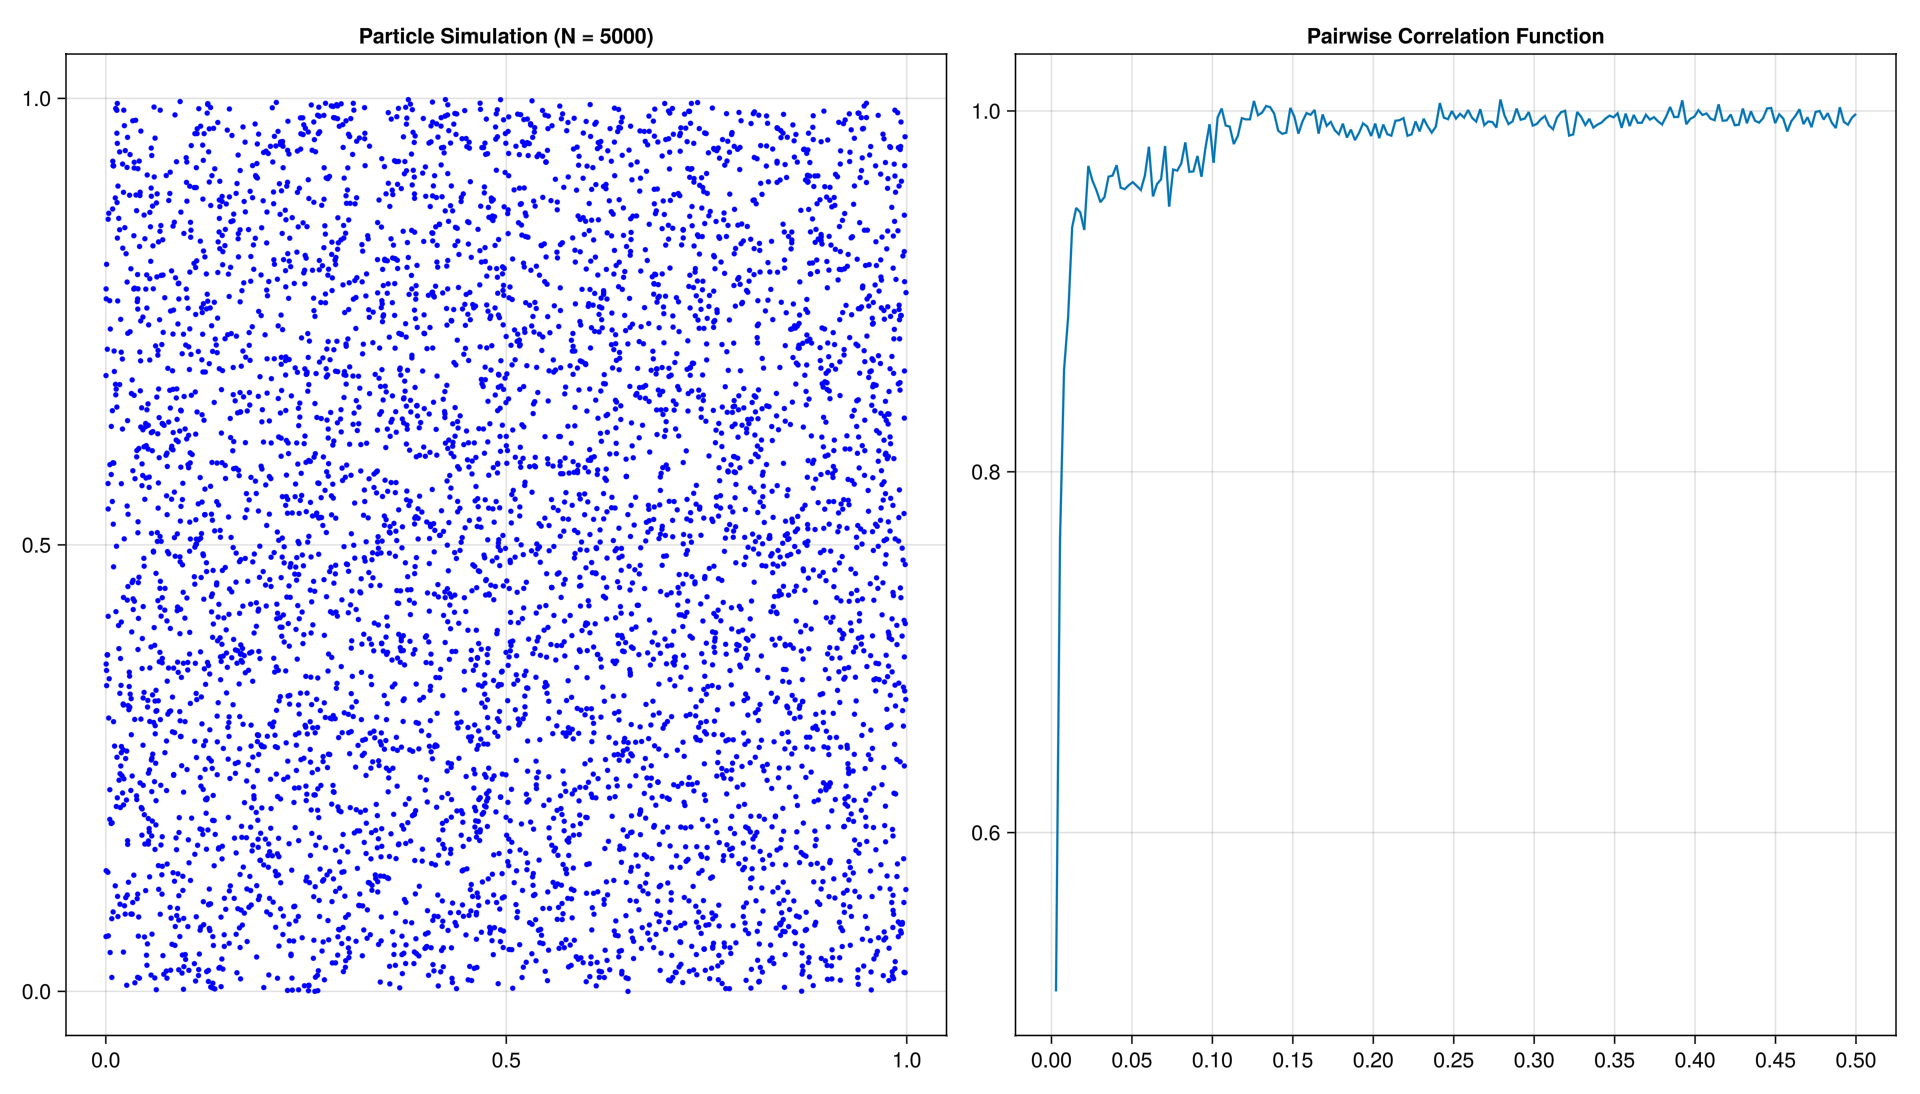
\includegraphics[width=1.0\linewidth]{img/rp151_N5000_D01_p4.png}
    \caption{Results of the simulation with $N=5000$, $p=4$, $D_0=0.01$. The left panel shows the final distribution of the organisms and the right panel shows the PCF of this configuration.}
\end{figure}
% clumped pattern
In Figure \ref{clumped}, a clumped configuration of organisms and the PCF can be seen, as before.
The clumps are very evenly spaced, forming a grid-like pattern. 
The PCF has clearly distinguished peaks and valleys, from which characteristic lengths in the system can be determined.
The first time the PCF drops below $1$ is for a distance slightly below $0.05$ and the PCF rises above $1$ for distances lightly above $0.1$, which is also the interaction range, $R$, of the organisms.
While for $N_2=1000$ a similar structure can be seen, just with fewer individuals per clump, for $N_1=200$ cluster sizes are so small (at most $3$ organisms), that no real patterns can be observed and the PCF is very noisy.
% resultplot 51 - 74 
\begin{figure}
    \label{clumped}
    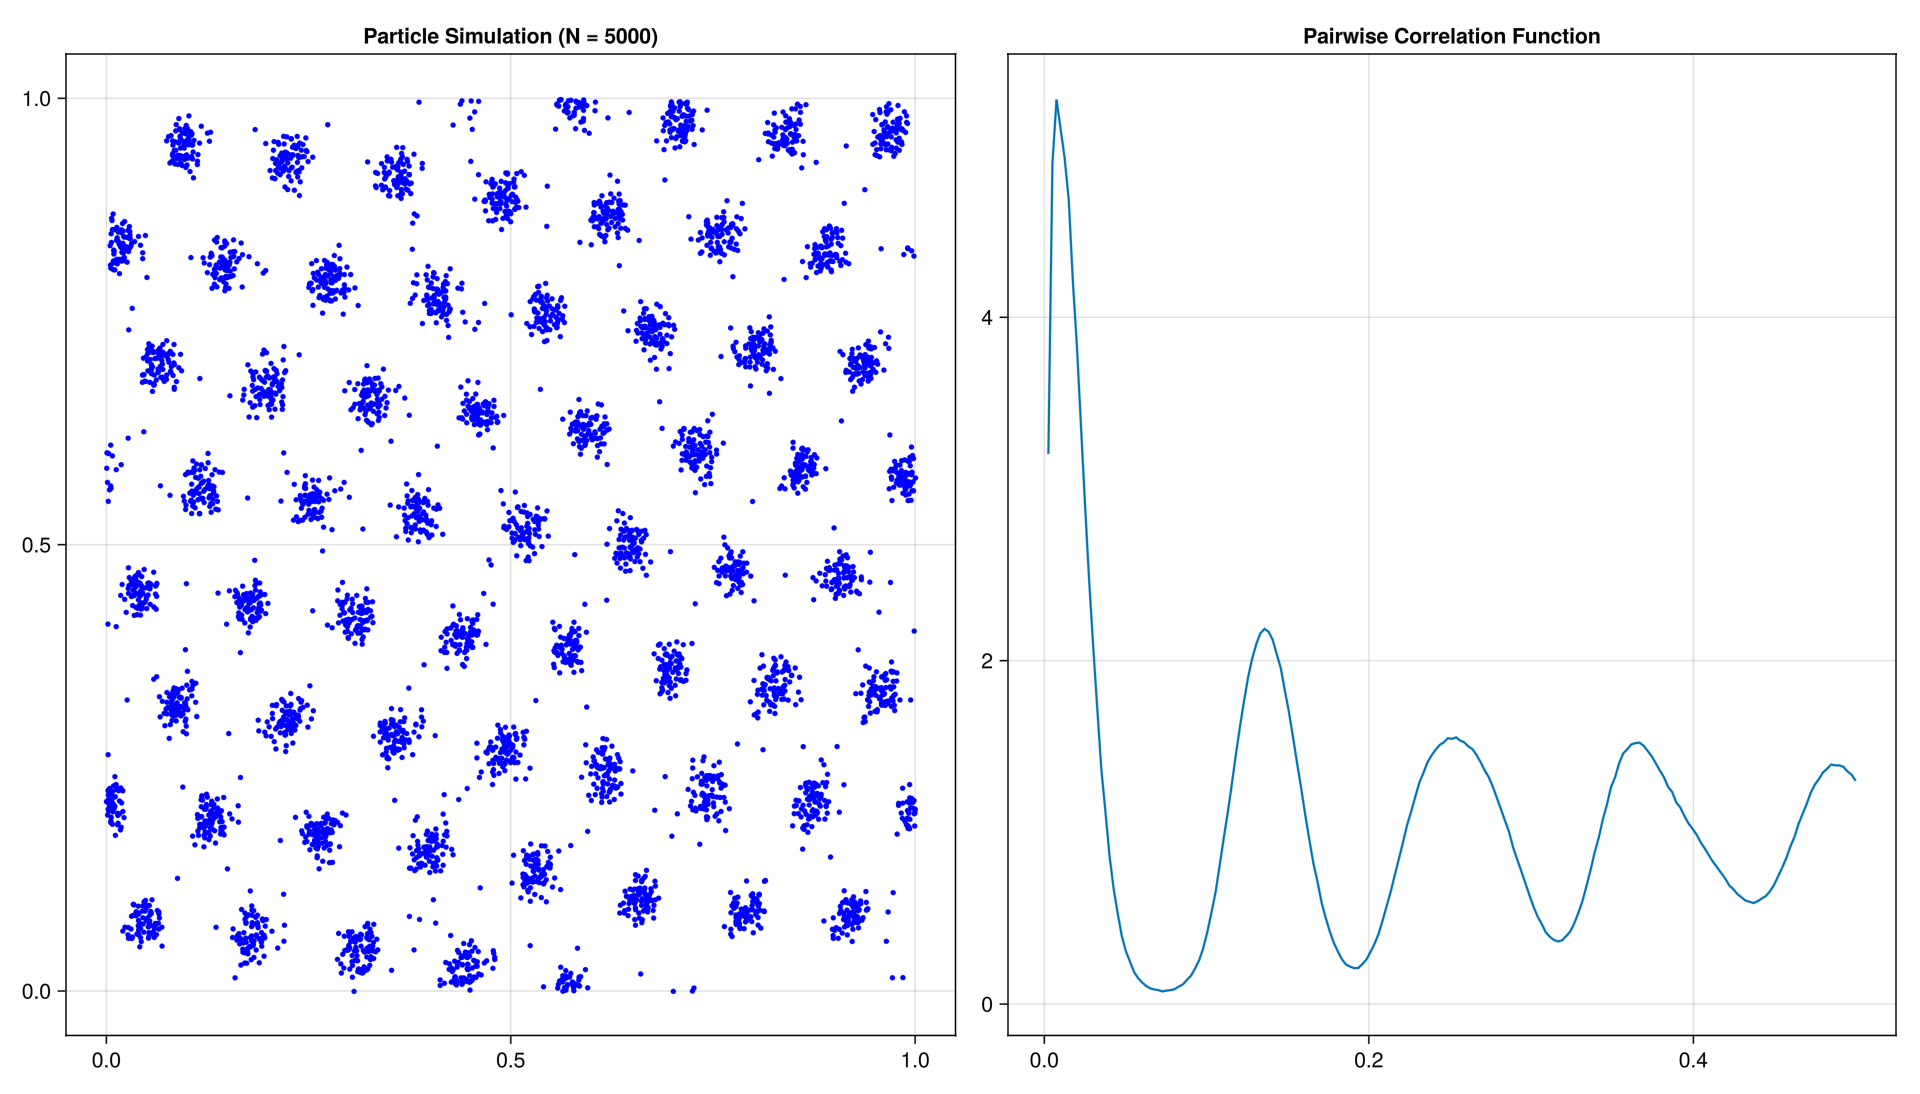
\includegraphics[width=1.0\linewidth]{img/rp68_N5000_D01_p8.png}
    \caption{Results of the simulation with $N=5000$, $p=8$, $D_0=0.01$. The left panel shows the final distribution of the organisms and the right panel shows the PCF of this configuration.}
\end{figure}

Using the property that the PCF is close to $1$ when the pattern is random and oscillates above and below $1$ when it is clumped, the MSD between the PCF and the line $g(d)\equiv 1$ is used as an indicator for how clumped the pattern is.
To find the range of parameters where clumped patterns occur, this indicator is calculated for a large number of parameters and plotted as a heatmap in Figure \ref{heatmap1000}. 
A slightly noisy transition occurs around $p=7$ from random to clumped but in contrast to what the stability analysis density-based approximation of this system predicts, there is clearly a dependence on the parameter $D_0$ as well. 
For large value of $D_0$, no clumped patterns occur anymore.
Additionally, very small values of $D_0$ also seem to lead to random patterns, however, this is an artifact of not running the simulation for long enough. 
In this case, the particle move very slowly and take much longer to settle into clumped patterns.
\begin{figure}
    \label{heatmap1000}
    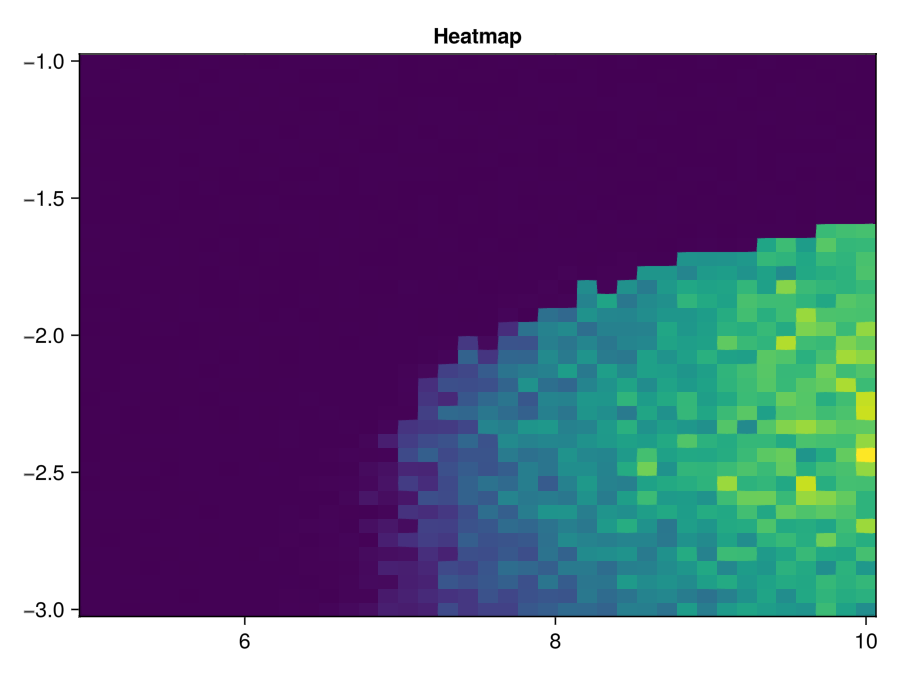
\includegraphics[width=0.9\linewidth]{img/heatmap1000.png}
    \caption{Value of the MSD between the PCF and $g(d) \equiv 1$ for a grid of parameter choices. Brighter values indicate clustering while dark purple means the final distribution of organisms was random.} 
\end{figure}

\section{Discussion}
We have seen a counter-intuitive mechanism that leads to pattern formation by organisms that move faster when more other organisms are around. 

Watching the simulation play out in real-time, helps in understanding why patterns can form through this counter-intuitive mechanism.
It boils down to a combination of a low baseline diffusion rate and a strong increase in the diffusion rate with a growing number of organisms within the interaction range.

A low baseline diffusion rate ensures that the clumps don't just diffuse away because the organisms move only slowly within clusters.
As we have seen in an earlier section, the mean displacement of an organism due to a constant diffusion rate grows like $2\sqrt{Dt}$. 
Thus an organism inside a cluster with an approximatly constant number of particles would leave the cluster after some amount of time, but this could take long time provided $D$ is small enough.

The second aspect allowing pattern formation is a rapid increase in the diffusion rate with an increasing number of organisms within the interaction range. 
As we have noted, clumps are slightly further apart than the interaction range, meaning that organisms within a cluster only interact within that cluster.
However, an organism that leaves the cluster through diffusion suddenly is within the interaction range of multiple clusters and has more organisms within their interaction range. 
Because the diffusion rate grows rapidly with an increase in neighbours, the organism moves very fast until it jumps into a cluster again where the diffusion rate becomes much lower again, because interaction occurs only within that cluster.
Since organisms take much longer to diffuse out of a cluster, than it takes them to be captured again, the clusters are stable.

% Additionally, the stability analysis indicates for which parameter values the initial uniform distribution becomes unstable, which allows clusters to form in the first place. 
% The onset of pattern formation already occurs for slightly smaller values of $p$ than the predicted value of $p_c =7.6$ where a transition region exists. 
% In this region, for example for $p=7.4$ and $D=0.01$, clusters start to form but dissolve again quickly and no stable pattern emerges.

While not being the focus of this report, a short discussion about the number of clusters and their distances is presented.
Without exactly measuring the size of clusters, they seem to have a diameter of around $0.04-0.05$ and the distance between clusters is around $0.12$, which indicates that clusters are spaced such that the organisms on the outer parts of a cluster already are within range of organisms of the next cluster. 
The clusters seem to be arranged along prallel lines and there are three directions of lines. 
Approximately $60-90$ clusters should be possible, meaning that for $1000$ organisms, the average cluster size is around $10-20$ organisms.
Importantly, the number of clusters and their distances does not seem to depend on the number of organisms.
Parameter choices that lead to clustering should have low diffusion rates while an organism is within the interaction range of a number of organisms that is around the average cluster size and then increase rapidly as the number of organisms within the interaction range grows to 2 times the average cluster size. 

This raises the question whether the same interaction range can lead to differently spaced and sized clusters or whether the interaction range forces a certain length scale on the system, and therefore also a certain average cluster population.

\printbibliography
\end{document}